\documentclass{report}


\usepackage{arxiv}

\usepackage[utf8]{inputenc} % allow utf-8 input
\usepackage[T1]{fontenc}    % use 8-bit T1 fonts
\usepackage{hyperref}       % hyperlinks
\usepackage{url}            % simple URL typesetting
\usepackage{booktabs}       % professional-quality tables
\usepackage{nicefrac}       % compact symbols for 1/2, etc.
\usepackage{microtype}      % microtypography
% figures
\usepackage{graphicx}
\usepackage{subcaption}
\usepackage[natbib=true,style=authoryear,maxnames=999,maxcitenames=2]{biblatex}
% tables
\usepackage{tabularx}
\usepackage{threeparttable}
\usepackage{multirow}
\usepackage{makecell}

% maths
\usepackage{amsfonts}       % blackboard math symbols
\usepackage{amsmath}
\usepackage{amssymb} %mathbb packages
\usepackage{siunitx}
\usepackage{algorithm, algorithmicx, algpseudocode}

\usepackage{pifont}
\usepackage{csvsimple}
\usepackage[title,toc,titletoc,page]{appendix}

% notes in the margin
\usepackage{todonotes}
\usepackage{snaptodo}

\setlength{\marginparwidth}{1.4cm}
\setlength{\marginparsep}{-.01cm}
%\setlength\textwidth{177.8mm}

\snaptodoset{block rise=1em}
\snaptodoset{margin block/.style={font=\tiny}} \newcommand{\gv}[1]{%
    \snaptodo[margin block/.append style=green!50!black]{%
	\sloppy\textbf{Gael}: #1}}
\snaptodoset{margin block/.style={font=\tiny}} \newcommand{\md}[1]{%
    \snaptodo[margin block/.append style=blue]{%
	\sloppy\textbf{Matthieu}: #1}}
  
% color commands
\colorlet{P}{ForestGreen}
\colorlet{I}{MidnightBlue}
\colorlet{C}{YellowOrange}
\colorlet{O}{DarkOrchid}

% equations commands
\newcommand{\indep}{\perp \!\!\! \perp}
\newtheorem{assumption}{Assumption}
\DeclareMathOperator*{\argmin}{argmin} \def\mycitecolor{green!50!black}
\usepackage{mathtools}
\newcommand\myeq{\stackrel{\mathclap{\text{def}}}{=}}

\bibliography{references} 


\title{
  Representations and inference from time-varying routine care data 
}

\author{Matthieu Doutreligne}
\date{}

\begin{document}
\maketitle

\begin{abstract}

  Real World Databases are increasingly accessible, exhaustive and with
  fine temporal details. Unlike traditional data used in clinical research, they
  describe the routine organization of care. These day-to-day records of
  patients care enable new research questions, notably concerning the efficiency
  of interventions after market access, the heterogeneity of their benefits in
  under-served populations or the development of personalized medicine. On the
  other hand, the complexity and large-scale nature of these databases pose a
  number of challenges for effectively answering these questions. To remedy
  these problems, econometricians and epidemiologists have recently proposed
  the use of flexible models combining causal inference with high-dimensional
  machine learning.

  Chapter 1 uses a national case study of the 32 French regional and
  university hospitals to highlight key aspects of modern Clinical Data
  Warehouses (CDWs), the cornerstone infrastructure of precision medicine. From
  semi-structured interviews and an analysis of declared observational studies
  on CDWs in France, I highlight both the current potential and challenges of
  leveraging these routinely collected data for research purposes.

  Acknowledging the difficulty to access large sample sizes and computational
  power to develop generalizable predictive models, Chapter 2 leverages
  distributional representations of medical concepts for clinical tasks. I show
  that these sharable representations out-perform more complex models for
  small sample datasets.

  Despite a current focus on artificial intelligence, healthcare does not seek
  purely predictive models, but appropriate interventions that will benefit
  specific patients. This is a decision making problem highly amenable to
  counterfactual prediction rather than statistical learning. Chapter 3 emulates
  a clinical trial to evaluate an intervention in the intensive care unit. I
  highlight the importance of the different practical choices when developing
  counterfactual prediction algorithms on time-varying data collected in routine
  care.

  In high-dimensional settings such as time-varying data and heterogeneity of
  interventions on subgroups, the selection of hyper-parameters for the causal
  model is crucial to avoid under- or over-learning. Chapter 4 demonstrates the
  fragility of the usual evaluation metrics (Mean Squared Error) for
  counterfactual predictions. I highlight the performance of the doubly robust
  R-risk over other existing risks and discuss their effectiveness regimes in a
  simulation and three semi-simulated datasets.

  Chapter 5 concludes by highlighting the potential of combining machine
  learning methods and routine care data to shed light on current public health
  issues. I discuss new avenues to improve the development and the evaluation of
  tailored interventions, public health policies or quality-of-care indicators.

\end{abstract}
% keywords can be removed
%\keywords{First keyword \and Second keyword \and More}

\tableofcontents




\chapter{Introduction: amazing opportunities of health data?}\label{chap:intro}
\section{How I came into this landscape}\label{sec:intro:landscape}

I will present my progression among these opportunities.

\subsection{Context: From a modern statistical formation to the first contact with epidemiology}\label{subsec:intro:context}

\paragraph{Learning statistics during the Natural Language Processing revolution}

Machine learning techniques, a subfield of artificial intelligence, became
increasingly good as solving complex tasks where previous pattern recognition
techniques were struggling. First, categorized into supervised and unsupervised
approaches, the pre-training paradigm became increasingly popular in the 2010's:
\cite{halevy2009unreasonable} proposed to take advantages of regularities
present in large piles of data to design automatically interesting features for
large application domains. The practical successes came in image processing
\citep{}, then Natural Language Processing \citep{} and structural biology.
%

\paragraph{APHP: Removing identification elements from clinical notes}

Continuous improvements in natural language processing led to the intuition that
soon the information contained in clinical texts could be mined by appropriate
to serve clinical research.

However, privacy concern: the access to very detailed elements of patient cares
is no more restricted to the medical staff.

Need for pseudonymization : use newly to reach State of the Art pseudonymization
\citep{dernoncourt2017identification, paris2019desidentification}.

\paragraph{Billing claims: an underused huge pile of data}

French ministry department of statistics had billions of claims extracted in a
dedicated server. But the amount of data made the job impossible.

I learned that distributed computing (aka appropriate tools), summary statistics
and good documentation.

I began to wonder what were the appropriate methodological tools to extract
relevant information from this data. Hammer that sees a nail : Can I use language
modeling techniques to mine this data ?

First questions: how useful are such wealth of data ? Is unsupervised learning
useful ? Is prediction a useful goal ? I was exactly in the atypical situation
mentioned by Cox in his answer to Breiman's foundational paper on Machine
Learning \citep{breiman2001statistical} : \textit{Data looking for a question are
  not unknown and raise puzzles but are, I believe, atypical in most contexts.}

Ironically, at the end of the day, I
replicated unsupervised learning results from \citep{beam2019clinical} but would
not know how to use it. I moved towards more interpretable dictionary learning
with control groups analyses to study polymedication.

% Not sure it is useful
Covid-19: National healthcare monitoring during the epidemics. Integrated data
pipeline are very useful during crisis for monitoring: If you do not see all the
data creating process, standard pipelines, standard tests and documentation : it
is inherently a group effort.

\subsection{Wrap-up: Increasing data collection and computing power}\label{subsec:intro:wrapup}

\paragraph{Data is collected at massive scale in healthcare} centralized
into dedicated databases for analysis: eg. APHP clinical notes, French.

It is acknowledged that we entered since at least 2022 years in an era where we
frenetically store data without having a dedicated question in mind. The vague
concept of big data describes this new attitude towards data collection. I would
propose another view on the current situation: data collected in huge quantity
is part of the reality, but it does not preclude to assemble data suited for an
appropriate question. In medical informatics, this is called computational
phenotyping.

\paragraph{Models are scaling up}
A whole generation of quantitative researchers has been trained with flexible
data-hungry models. The unreasonable effectiveness of data \citep{halevy2009unreasonable}.

A recent work on the classification of data and models (AI) in clinical medicine
suggests three main usages: AI in clinical practice, clinical research on AI/ML
device and applications and AI/ML used to conduct clinical research
\citep{haug2023artificial}.

\subsection{What pressing needs to use health data}

Shortliffe, the inventer of MYCINE \citep{shortliffe1974mycin}, the first
rule-based artificial intelligence expert systems described \textit{medical
  practice, and biomedical research, [as] inherently information-management tasks}
\citep{patel2009coming}.

However, the incentives to collect and analyze data are not aligned between
healthcare actors.

\paragraph{Healthcare practice}

Automation of tedious tasks, decision support system

\paragraph{Research}

Drug development, evidence based medicine, biomarkers, epidemiology ie.
understanding of the mechanisms of disease \textit{the study of the distribution
  and determinants of disease frequency} \citep{macmahon1970epidemiology}

\paragraph{Public policies: monitoring and evaluation}

Guidelines, quality of care, public health

Health Technology Agencies interest: organizational impact of health products,
potential for real world efficiency (entire life cycle of the product), quality,
security, pertinence and security of care,

Government bodies: health monitoring, health management, contextualization.

% I am not totally naive
\paragraph{Marketing}

Market access, tailored recommendations.

\section{The data: Electronic Health Records}\label{sec:intro:data}

\subsection{Various types of data: Real World Data}\label{subsec:intro:real_world_data}

Real world data refer to routinely collected data

Gradient and distinction between research data and opportunistic data
collection.

\paragraph{Traditional research data collections}

Hand made data collection for one research question with a specific protocol,
Specialized registry and cohorts


\paragraph{Claims}

Billing system, eg. PMSI.

Advantages (space and time coverage, scale, structure), disadvantages (not clinic, no exam results, few measures, heterogeneity of collection)

\paragraph{EHRs and Hospital Information System}

Increasing informatization
EHR at the center
Other applications part of HIS: give examples.

\subsection{Interventional data vs observational
  data}\label{subsec:intro:interventional_vs_observational}


Interventional data contains interaction with the patients / environment where
the intervention probabilities are known. Eg. RCT : fixed probability for any
patient (statistical unit): first RCT, RCTs as the basis of Evidence Based
Medicine in the late 80s.

\textit{In an experiment, the reason for the exposure assignment is solely to
  suit the objectives of the study; if people receive their exposure assignment
  based on considerations other than the study protocol, it is not a true
  experiment} \citep{rothman2012epidemiology}

Pbs of external validity raised in economics (Deaton, cf intro de la revue de
Bénédicte). Focus is such problems is probably greater in economics because
situations are not well controlled at all: very far from labs settings. Clinical
situation is closer to lab (clinical epidemiology != social epidemiology). What
about medico-economics ? I do not address this question in the present thesis,
but it is a clear motivation.

%
Observational data cannot intervene in any way with the patients. It should rely
on observation alone to estimate intervention probability.

% Interventional vs Observational: A gradient as well 
Conditional probabilities are interventional as well: conditionally randomized
experiments in epidemiology \citep{hernan2020causal}. This concept is known as
reinforcement learning in the Machine Learning community (bareinboim2015bandits)
where intervention probabilities are known \cite{bareinboim2015bandits}.
Decision making processes rely to the correct estimations of these
conditional probabilities, hence the link between this work and precision medicine.

\subsection{Focus of this thesis: real world data, observational}\label{subsec:intro:focus_data}

Inconvenient of interventional data : Increasing costs of RCTs,

Today's public health issues are closely linked to routine care, not ideal care:
resource constraint, chronic disease. Not so new as it was already major issues
mentioned in the late 60s \cite{rutstein1967coming}: \textit{1) modern
  medicine's skyrocketing costs; 2) the chaos of an information explosion
  involving both paperwork proliferation and large amounts of new knowledge that
  no single physician could hope to digest; 3) a geographic maldistribution of
  MD's; 4) increasing demands on the physician's time as increasing numbers of
  individuals began to demand quality medical care.}

Rise of digitalization and computing power suggesting new research methods

\section{Two cultures of statistics for health}\label{sec:intro:two_cultures}

In 2001, \cite{breiman2001statistical} clearly separates two statistical
cultures: a predominant community at the time focused on models, another one
relying on predictive accuracy.

Epidemiological statistics tends to be closer to the first model-based culture
whereas artificial intelligence in medicine embraced the second one. This
cultural differences might be explained by different objectives. Clinical
Epidemiology seeks to uncover nature mechanisms from data, to understand how
nature works. AIM adopts a more pragmatic approach, trying to understand what
deployed healthcare system is improving outcomes or not, without trying to
uncover the full causal mechanism leading to observed results.

\begin{baground_box_left}
  \subsection{Machine Learning Framework}\label{subsec:intro:machine_learning}

  Departing from carefully designing functional forms for statistical models,
  seeking algorithm efficiency and out-of sample predictive accuracy.

  \paragraph{Rashomon effect: multiple models can equally well model a given dataset}
  % ref to appendix to describe ML algorithms: at least ridge, random forest, boosting.

  \paragraph{Model selection}
  Hyper-parameters selection, cross-validation (stone, 1974) and Textbook figure

  \subsection{Biostatistics Framework}\label{subsec:intro:biostatistics_framework}

  In medical journals, Cox model for survival data and logistic regression for
  binary outcomes have been the standard for publication.

  Focus on variable selection: root in hand collected variables in carefully
  designed subpopulation ?

  Focus on simple models for juridical and credibility reasons but also for
  practical reasons: the input data should be readily available to question one
  model individual prediction \citep{wyatt1995commentary}.

  The divide between modeling and empirical algorithmic approaches is best
  illustrated in the commentary to Breimann by David Cox or Bad Efron in  \cite{}:

  \textit{Often the prediction is under quite different conditions from the
  data; [...] what would be the effect on annual incidence of cancer in the
  United States of reducing by 10\% the medical use of X-rays}. This example is
  a pure causal inference question.

\end{baground_box_left}

\subsection{One choice of perspective: Recent statistical
  learning}\label{subsec:intro:recent_statistical_learning}
% 
\paragraph{This perspective reflects more naturally my progression:} Learning
statistics in the age of deep learning pushes towards adopting a view on
statistics that consider mechanisms as generally unknown, and predictive
accuracy as the hallmark of validity \citep{breiman2001statistical}.
% 
% ML in healthcare 
\paragraph{Recent discourse and successes are heavily influenced by this line of
  though:} Machines read medical images faster and more efficiently than most
practitioners \citep{zhou2021review}. Structured data from Electronic Health
Records \citep{rajkomar2018scalable} or administrative databases
\citep{beaulieu2021machine} outperform rule-based clinical scores in
predicting patient's readmission, in-hospital mortality or future
comorbidities \citep{li2020behrt}. Recently, large language models (LLMs)
leveraged clinical notes from several hospitals for length of stay prediction
\citep{jiang2023health}. Hope is high that LLMs models will soon be able to
help practitioners during consultation \citep{lee2023benefits}.


\section{Notions of causality}\label{sec:intro:causality}

\begin{baground_box_left}

  \subsection{Association is not causation}\label{subsec:intro:causation}

  \paragraph{Observational data can have different causal interpretations}

  One statistical model yields multiple causal models, only one of which
  correctly reflects the reality : find a good medical example (otherwise look
  into Peter jonas's book or \cite[chapter~36]{murphy2022probabilistic}).

  \paragraph{Causality in epidemiology}

  Opening an epidemiological book, confounding is the very first explained concept
  \citep{rothman2012epidemiology}.

  Causes are mainly presented as binary variables absent or present in \citep{}.
  Their strengh is only defined at a population level, making them relative to a
  given population \citep[chapter~3]{rothman2012epidemiology}. This point of
  view is rather aligned with statistical modeling related to variable
  significance, not with model performances.

  Interesting concept of promoter --the last component cause-- that

  Importance of validity by generalization of theory rather than statistical
  generalization: established epidemiological knowledge should \textit{tell us
    what to expect in people or settings that were not studied.} Statistical
  generalization is considered by \cite{rothman2012epidemiology} as applied
  epidemiology, focused on specific cases and not as the core of epidemiological
  science.

  \paragraph{Causality in Machine Learning}

  Relation to dataset shift \citep{subbaswamy2020development}

  Distinction between association and causation (ladder of causation): first
  insight that different tools than statistics are needed.


  \subsection{Neyman-rubin causal framework}\label{subsec:intro:causal_framework}

  - PO notations
  - Explain what is a rct, its origin and the difference with an observational study
  - Send back to appendix the Difference in Means  (in randomized experiments)
  - The rest will be presented in chapter 4 and 5.

\end{baground_box_left}

\section{Overview and contributions}\label{sec:intro:contributions}



\chapter{Potential and challenges of Clinical Data Warehouse, a case study in France}\label{chapter:cdw}

\section{Abstract}\label{sec:cdw:abstract}
\section{Motivation and background: A changing world}\label{sec:cdw:motivation}

\subsection{Data for primary or secondary
  usages?}\label{subsec:cdw:data_usages}

\paragraph{Primary data usages}
Primary usages directly serve one patient care.

\paragraph{Secondary data usages}
Secondary usages do not concern directly the care and support of one patient:
research, quality or management indicators, billings.

\paragraph{Towards mix usages: the learning health system paradigm}

The notion of learning health system \citep{mcginnis2013best}.

Mix usages such as learning algorithms

\subsection{Healthcare data collection is heavily influenced from the local healthcare organization}

\paragraph{Centralized data collections: ex. Israël, HIRA}

\paragraph{More heterogeneous data collections structured into networks} ex. from

US, Korea, Germany,

\paragraph{The case of France}

centralized national insurer but scattered hospital ehrs. Projects in other areas: eg. cancer (unicancer), gp (cnge project, darmoni). National initiative to develop and structure hospital cdws.

\subsection{The multiplication of Clinical Data Warehouses}\label{subsec:cdw:cdw_definition}

An infrastructure is needed to pool data from one or more medical information
systems. Definition of Clinical Data Warehouse: Health data warehouses (HDWs)
refer to the pooling of data from one or more medical information systems, in a
homogeneous format for reuse in management, research or care.


The 4 phases of data flow from the various sources that make up the HIS (figure)
Focus of this thesis: Clinical Data Warehouse and EHR, though most of my work should apply to claims


\section{Speaking to the data collectors: Interviews of French
  University Hospitals}\label{sec:cdw:methods}

\subsection{Interviews and study coverage}\label{subsec:cdw:interviews}

\paragraph{Semi-structured interviews}

Topics, questions, link to full data and questionnaires in appendix.

\paragraph{Regional and university hospitals in France: different levels of maturity}

Scope of 32 CHUs, out of the 3000 care sites in France to yield exhaustive
conclusion on a restricted scope. Drive most specialized care, research in their
core mission. Date of interview

\paragraph{Focus on the 18 CDWs with highest level of maturity}

The denominator for the quantitative results is the 18 CDWs in production

\subsection{A classification of observational
  studies}\label{subsec:cdw:classification}

Contrast with classical epidemiology study types and the notion of experiment \citep{rothman2012epidemiology}.

\paragraph{Outcome frequency}
\paragraph{Population characterization}
\paragraph{Risk factors}
\paragraph{Treatment effect}
\paragraph{Development of diagnostic or prognostic algorithms}
\paragraph{Medical informatics}


\section{Observations from a rapidly evolving and heterogeneous
  ecosystem}\label{sec:cdw:results}

\subsection{Governance: CDW are federating multiple teams in the
  hospital}\label{subsec:cdw:results:governance}
\paragraph{Initiation and actors}
Figure temporality of CDW
Federating potential
Multiple departments involved
Multiple skills involved, strong ties with the academics
In-house solution development vs industrialization

\paragraph{Management of studies}

Scientific committee and project follow-up platform

\subsection{Uneven transparency of ongoing
  studies}\label{subsec:cdw:results:transparency} Uneven public reference on
hospital websites of ongoing studies.

\subsection{Triple usage of data: Research, management,
  clinic}\label{subsec:cdw:results:data}

\paragraph{Strong dependance to the HIS}

Data collected reflect data collection
Exemples, AP-HP, HCLs

\paragraph{Categories of Data}

Main functionalities of HIS are the same. Common base Details: Table Takeaway:
most of the current accessible data are billing, administrative and text,
importantly, low access to temporality.

\paragraph{Data reuse: Research}
Details of current study types.
Details of specialty of the principal investigator
Interest for research data network but lack of resources

\paragraph{Data reuse: CDW are used for monitoring and management}
Initialization for billing
Potential for professional feedbacks
Pharmacovigilance

\paragraph{Data reuse: Strong interest for CDW in the context of care}

Some CDWs develop specific applications that provide new functionalities
compared to care software. Search engines can be used to query all the
hospital's data gathered in the CDW, without data compartmentalization between
different softwares. Dedicated interfaces can then offer a unified view of the
history of a patient's data, with inter-specialty transversality, which is
particularly valuable in internal medicine. These cross-disciplinary search
tools also enable healthcare professionals to conduct rapid searches in all the
texts, for example, to find similar patients \citep{garcelon2017finding}.
%
There is a growing interest in such computational phenotyping tools to support
the development of digital health solutions \citep{wen2023impact}.
%
Uses for prevention, automation of repetitive tasks, and care coordination are
also highlighted. Concrete examples are the automatic sorting of hospital
prescriptions by order of complexity or the setting up of specialized channels
for primary or secondary prevention.

\subsection{A multi-layered technical
  architecture}\label{subsec:cdw:results:architecture} Three layer : Data
preprocessing (acquisition and normalization), storage, exposure Datalab: a
crucial technological brick

\subsection{Too little data quality and too many data
  formats}\label{subsec:cdw:results:data_quality}
\paragraph{Quality tools}
Automatic tooling for acquisition
First development for automatic data checks
\paragraph{Standard format}
No single standard data model,
Omop
eHop
\paragraph{Documentation}
Half of the CDWs have put in place documentation accessible within the organization
No documentation is public

\section{Recommendations: How to consolidate EHRs and expand
  usages}\label{sec:cdw:recommendations}

\subsection{Governance: CDWs are
  infrastructures}\label{subsec:cdw:recommendations:governance}

CDW becomes an essential component of data management in the hospital Resources
specific to the warehouse are rare and only project-based. Should promote
long-middle term teams (eg. inria ?) Multi-layered governance

\subsection{Transparency: Keep the bar
  high}\label{subsec:cdw:recommendations:transparency} Public registration of
comparative observational study protocols for research Patient information stays
limited

\subsection{Data: Complex data collection requires a variety of
  expertise}\label{subsec:cdw:recommendations:data} study design : change of
focus from data collection to data preprocessing -> other complementary skills
needed Link with the HIS, lack of standard at the HIS level, lack of sharing of
data schema Data reuse oriented towards primary care is still rare and rarely
supported by appropriate funding.


\subsection{Technical architecture: Towards more harmonization and open source ?
}\label{subsec:cdw:recommendations:architecture} Lack of harmonization: focus on
fewer solutions Commercial solutions emerging Case for open source:
transparency, less technological lock-in, mutualization, favor modularity, help
build consensus Opportunity for open source solutions Data quality, standard
formats Quality is not sufficiently considered as a relevant scientific topic
itself. Tooling: Link with devops/ automated CI in industrial data science there
is a need for open-source publication of research code to ensure quality
retrospective research

\subsection{Data quality an document: more incentives needed}\label{subsec:cdw:recommendations:quality}

Quality is not sufficiently considered as a relevant scientific topic itself.
However, it is the backbone of all research done within a CDW. In order to
improve the quality of the data with respect to research uses, it is necessary
to conduct continuous studies dedicated to this topic [52,54–56]. These studies
should contribute to a reflection on methodologies and standard tools for data
quality, such as those developed by the OHDSI research network [41].

Finally, there is a need for open-source publication of research code to ensure
quality retrospective research [55,57]. Recent research in data analysis has
shown that innumerable biases can lurk in training data sets [58,59]. Open
publication of data schemas is considered an indispensable prerequisite for all
data science and artificial intelligence uses [58]. Inspired by data set cards
  [58] and data set publication guides, it would be interesting to define a
standard CDW card documenting the main data flows.

\section{Conclusion}\label{sec:cdw:conclusion}

The French CDW ecosystem is beginning to take shape

The priority is the creation and perpetuation of multidisciplinary warehouse teams

Constitution of a multilevel collaboration network is another priority.

Common data model should be encouraged

The question of expanding the scope of the data beyond the purely hospital domain must be asked.

Heterogeneity of data collection calls for distributed information sharing models.

\chapter{Exploring a complexity gradient in representation and predictive algorithms for EHRs}\label{chapter:predictive_models}
\section{Abstract}\label{sec:predictive_models:abstract}

\section{Predictive models in healthcare: Less fascination, more practical utility}\label{sec:predictive_models:motivation}

\subsection{Why such interest in predictive models in healthcare}\label{subsec:predictive_models:importance}

\paragraph{Interest in the clinic}

% better use of constrained medical resources
\textit{Being able to predict key outcomes could, theoretically, make the use of
  hospital palliative care resources more efficient and precise} \citep{topol2019high}

The Framingham risk score, one of the earliest predictive model in medicine was
designed to predict Coronary heart disease risk by fitting a cox model using
seven features on 5300 patients: age, cholesterol, systolic blood pressure,
hematocrit, ECG status, smoking at intake, and relative body weight
\citep{brand1976multivariate}.

\cite{harrell2001regression} mention diagnosis, prognosis, confounder adjustment
and heterogeneous treatment effects (mainly for cost-effectiveness analyses) as
the main uses of predictive models in healthcare. Ten years later,
\cite{steyerberg2009applications} also mentions diagnosis, prognosis and therapy
(He has a great figure from pubmed). I should do the same for 2023.

Some are used in clinical practice every day : the Glasgow coma scale
\citep{teasdale1974assessment}, the APACHE III score \citep{knaus1991apache}.
But a very small part of the published models are used in practice
\citep{wyatt1995commentary}. Reasons for this poor adoption are lack of
evidences for credibility, generalizability or clinical effectiveness.

Prevention : \textit{Early detection and appropriate treatment of sepsis have
  been associated with a significant mortality benefit in hospitalized patients}
\citep{wong2021external}

Alert systems \citep{yu2018artificial}.

Patient deterioration detection \citep{rothman2013development}: \textit{Rather than attempting to forecast a particular
  adverse event, we argue that intervention during early deterioration can help prevent such an adverse event from
  occurring}

\paragraph{Risk stratification}

risk stratify \citep{tang2007global}

\paragraph{Long term prevention}


\paragraph{Planning and piloting}

Rejoin the logistic and administrative help from \cite{topol2019high}.

The LOS task: planning the number of beds and members of staff required,
identifying individual outliers and case mix correction for benchmarking \citep{verburg2017models}

\paragraph{Exploring french CDWs:} 23 \% of studies, just after population definitions).

\subsection{Data sources fueling predictive models are increasingly complex}\label{subsec:predictive_models:complex_data}

Why is EHR so complex ? How ? time, high cardinality, multi-modality

\paragraph{In the literature}: early article in \cite{wu2010prediction},
literature review from 2017 \citep{goldstein2017opportunities}, literature
review more focused on models and task from soda prez.

Within french CDW(link with previous chapter)

\subsection{Low prevalence and local practice: Headaches for machine learning}\label{subsec:predictive_models:low_prevalence}

For logistic models, a requirement is that the test set should have at least 10
cases per feature with a positive event (eg. mortality)
\citep{harrell1985regression,wyatt1995commentary}.

\subsection{What makes a healthcare predictive model useful?}\label{subsec:predictive_models:useful}

What are the most impactful algorithms for predictive tasks from structured EHR
? A wealth of methods, but a lack of insights on the advantages and
inconvenience for specific problems and resources.

We build upon the criteria for adoption from \cite{wyatt1995commentary}.

More modern sources eg. \cite{subbaswamy2020development}.

\paragraph{We can share it easily: } Hence, people can use it AND contribute to
external validity and continuous improvements.

\paragraph{Performances} linked to accuracy, but questions on how to measure it.

\paragraph{Insertion in the care workflow}

Arguments for ease of deployment.

\section{From basic to complex: four increasingly sophisticated predictive pipelines}\label{sec:predictive_models:pipelines}

\subsection{Demographic features}\label{subsec:predictive_models:demographic}

\subsection{Count encoding with event features}\label{subsec:predictive_models:count_encoding}

\subsection{Static Embeddings of event features}

\subsection{Transformer based}\label{subsec:predictive_models:transformer}

\section{Empirical Study}\label{sec:predictive_models:empirical_study}

\subsection{Evaluation pipeline}\label{subsec:predictive_models:evaluation_pipeline}

\subsection{Three clinical and operational tasks}\label{subsec:predictive_models:task_definitions}

\paragraph{Length Of Stay: Plan}

\paragraph{Diagnosis Prediction: Benchmark}

\paragraph{Major Adverse Cardiovascular Events: Prevent}

\subsection{Results: Performance-sample trade-offs}

\section{Conclusion}\label{sec:predictive_models:conclusion}

\chapter{Prediction is not all we need: Causal analysis of EHRs to ground decision making}\label{chapter:causal_tuto}
\section{Abstract}\label{sec:causal_tuto:abstract}

\section{Motivation : Healthcare is concerned with decision making, not mere
  prediction}\label{sec:causal_tuto:motivation}


Even the early Framingham study concludes that risk reduction is more important
than identifying the strength of specific risk factors since this quantity is
subject to slight changes in the risk model \citep{brand1976multivariate}:
\textit{It further suggests that the strength of a particular risk factor may
  not be as important from the point of view of intervention as the ability to
  safely and conveniently achieve even a moderate risk reduction in a large number
  of persons.}
In a foundational article on EHR, the use-case of heart failure prediction is
motivated by agressive interventions \citep{wu2010prediction}: \textit{heart
  failure could potentially lead to improved outcomes through aggressive
  intervention, such as treatment with angiotensin converting enzyme
  (ACE)-inhibitors or Angiotensin II receptor blockers (ARBs).}. It is almost
always the case that prognosis models are motivated by decision making
processes. It is clearly described by \cite{steyerberg2009applications} for
diagnosis: \textit{If we do a diagnostic test, we may detect an underlying
  disease. But some diseases are not treatable, or the natural course might be
  very similar to what is achieved with treatment.}

\subsection{Predictive medicine currently suffers from
  biases}\label{subsec:causal_tuto:predictive_medicine_biases} (shortcuts,
population shifts). Racial, gender and under-served population biases raise
concern on fairness.
\subsection{A key ingredient to ground data-driven decision making is causal thinking}

\subsection{The need for synthetic materials for practitioners}\label{subsec:causal_tuto:synthetic_materials}

The relevant concepts for causal inference are scattered in different literatures. A dedicated exposition to time-varying data in EHRs would help practitioners and data scientists that study them.
\subsection{Motivating example}\label{subsec:causal_tuto:motivating_example}


\section{Step-by-step framework for robust decision making from EHR data}\label{sec:causal_tuto:framework}

\subsection{Robust study design to avoid biases: Framing the question}
PICOT
Selection Bias
Immortal time bias

\subsection{Is the dataset sufficient to inform on the intervention: identification}
Causal graph Computing the causal effect of interest: Estimation Confounders
extractions Confounders aggregation Causal estimators Nuisance estimators
\subsection{Assessing the robustness of the hypothesis: Vibration or sensitivity
  analysis}\label{subsec:causal_tuto:vibration_analysis}

Sensitivity vs robustness

\subsection{Heterogeneity of treatment}

Interest of HTE
How to do HTE ? Final regression analysis.

\section{Application on MIMIC-IV}\label{sec:causal_tuto:application}

Emulated trial: Effect of albumin in combination with crystalloids compared to crystalloids alone on 28-day mortality in sepsis patients
Choice of the trial
Known effects

\subsection{Framing the question}\label{subsec:causal_tuto:framing_mimic}

\subsection{Identification}
Covariates and dag

\subsection{Estimation}
Confounders extractions
Confounders aggregation
Causal estimators
Nuisance estimators

\subsection{Vibration analysis}
Varying estimation choices:
Varying inclusion criteria: illustration of immortal time bias

\subsection{Heterogeneity of treatment}

\section{Discussion}\label{subsec:causal_tuto:discussion}

\chapter{How to select predictive models for causal inference?}\label{chapter:causal_model_selection}
\section{Abstract}\label{sec:causal_model_selection:abstract}

\section{Motivation}\label{sec:causal_model_selection:motivation}

\subsection{Extending prediction to prescription needs causality}

\md{watchout that I did not say the same thing as in chapter 4}
Progress in machine learning brings predictive models to new health
data \citep{beam2018big,rajkomar2019machine}, with the promise of
precision medicine.
Automated analysis of
medical images is increasingly accurate, \emph{eg} for brain images,
\citep{khojaste2022deep,zhang2019radiological} or mammography
\citep{yala2019deep,shen2019deep,nassif2022breast}.
New prognostic models leverage routinely-collected
patient records
\citep{mooney2018bigdata}: predicting heart
failure from claims \citep{desai2020comparison}, suicide attempts
from questionnaires \citep{simon2018predicting}...
Clinical notes contain much prognostic information
but require text modeling  \citep{horng2017creating,wang2020prediction,spasic2020clinical}.
Data may be difficult to
control and model, but the accuracy of the prediction can be verified
on left-out data
\citep{altman2009prognosis,poldrack2020establishment,varoquaux2022evaluating}.
Given a model predicting a health outcome, precision medicine
would like it to guide decisions: will an individual benefit from an
intervention such as surgery \citep{fontana2019can}?
Contrasting predictions with and without the treatment gives an answer,
but statistical validity requires causal inference
\citep{snowden_implementation_2011,blakely2020reflection}.

% - Causal inference is difficult
% - Beyond the dream of assessing effectiveness and safety in real-word
%   practice \citep{black1996we} include off-label drug usage 
%   \citep{radley2006off} (which may lead to drug repurposing)
% - Plug in that outcome modeling is complementary to RCTs: observational
%   data gives weaker evidence than trials, but on both data outcome
%   modeling opens the door to individual.
% - Epidemiology has focused on propensity-score methods
% - Principle causal inference with outcome models is possible
% - It brings the promises of \emph{individualized treatment effects} --a
%   goal related to capturing heterogeneity and thus CATE--
% - It also performs well on causal-inference competition, although they
%   focused on the ATE

% The plethora of approaches approaches give different causal-inference
% estimates => need for guideline on causal model selection.

There is a rich causal-inference statistical literature, which bridges to
predictive modeling via so-called \emph{outcome models}, or G-computation,
G-formula \citep{robins_role_1986}, Q-model \citep{snowden_implementation_2011},
conditional mean regression \citep{wendling_comparing_2018}. A central challenge
of inference of treatment effects is that of confounding: spurious associations
between treatment allocation and baseline health, \emph{eg} only prescribing a
drug to mild cases \citep{hernan_causal_2020,vanderweele2019principles}.
Controlled allocation of treatment, as in randomized controlled trials (RCTs),
alleviate this concern. Yet most machine-learning models are trained on
\emph{observational} data, close to real-word practice
\citep{black1996we,hernan_methods_2021} but challenging for causal inference.
Causal inference has been central to epidemiology, typically with methods that
model treatment assignment \citep{austin_moving_2015,grose_use_2020}, based on
propensity scores \citep{rosenbaum_central_1983}. Recent empirical results
\citep{wendling_comparing_2018,dorie_automated_2019} show benefits of outcome
modeling to estimate average treatment effects. Maybe a greater benefit is
that these methods naturally go beyond average effects, estimating
individualized or conditional average treatment effects (CATE), central to
precision medicine.
%
For this purpose, such methods are also invaluable on randomized trials
\citep{su2018random,lamont2018identification,hoogland2021tutorial}.

%\idea{There is a variety of models for g-estimation}
There is an explosion of outcome modeling or machine learning methods.
For instance, many deep-learning methods have been developed for medical
image analysis \citep{shen2017deep,monshi2020deep}.
Even outcome-modeling methods specifically designed for causal
inference are numerous: Bayesian Additive Regression Trees
\citep{hill_bayesian_2011}, Targeted Maximum Likelihood Estimation
\citep{laan_targeted_2011,schuler_targeted_2017}, causal boosting
\citep{powers_methods_2018}, causal multivariate adaptive regression
splines \citep{powers_methods_2018}, random forests
\citep{wager_estimation_2018, athey_generalized_2019},
Meta-learners \citep{kunzel_metalearners_2019}, R-learners
\citep{nie_quasioracle_2017}, Doubly robust estimation
\citep{chernozhukov_double_2018}...
%\idea{The variety of estimators calls for model selection procedures}
The wide variety of methods raises the problem
of selecting between different estimators based on the data at hand.
%
Indeed, estimates of treatment effects can vary markedly across different
predictive models. For instance, Figure shows
large variations obtained across different outcome estimators on
semi-synthetic datasets \citep{dorie_automated_2019}. Flexible models
such as random forests are doing well in most settings except
when treated and untreated populations differ noticeably, in
which case a linear model (ridge) is to be preferred.
However random forests with different hyper-parameters
(max depth= 2) yield poor estimates.
A simple rule of thumb such as preferring flexible models does not work in
general; model selection is needed.

%\idea{It is crucial to have tools for model selection.}

\begin{figure}
  \centering
  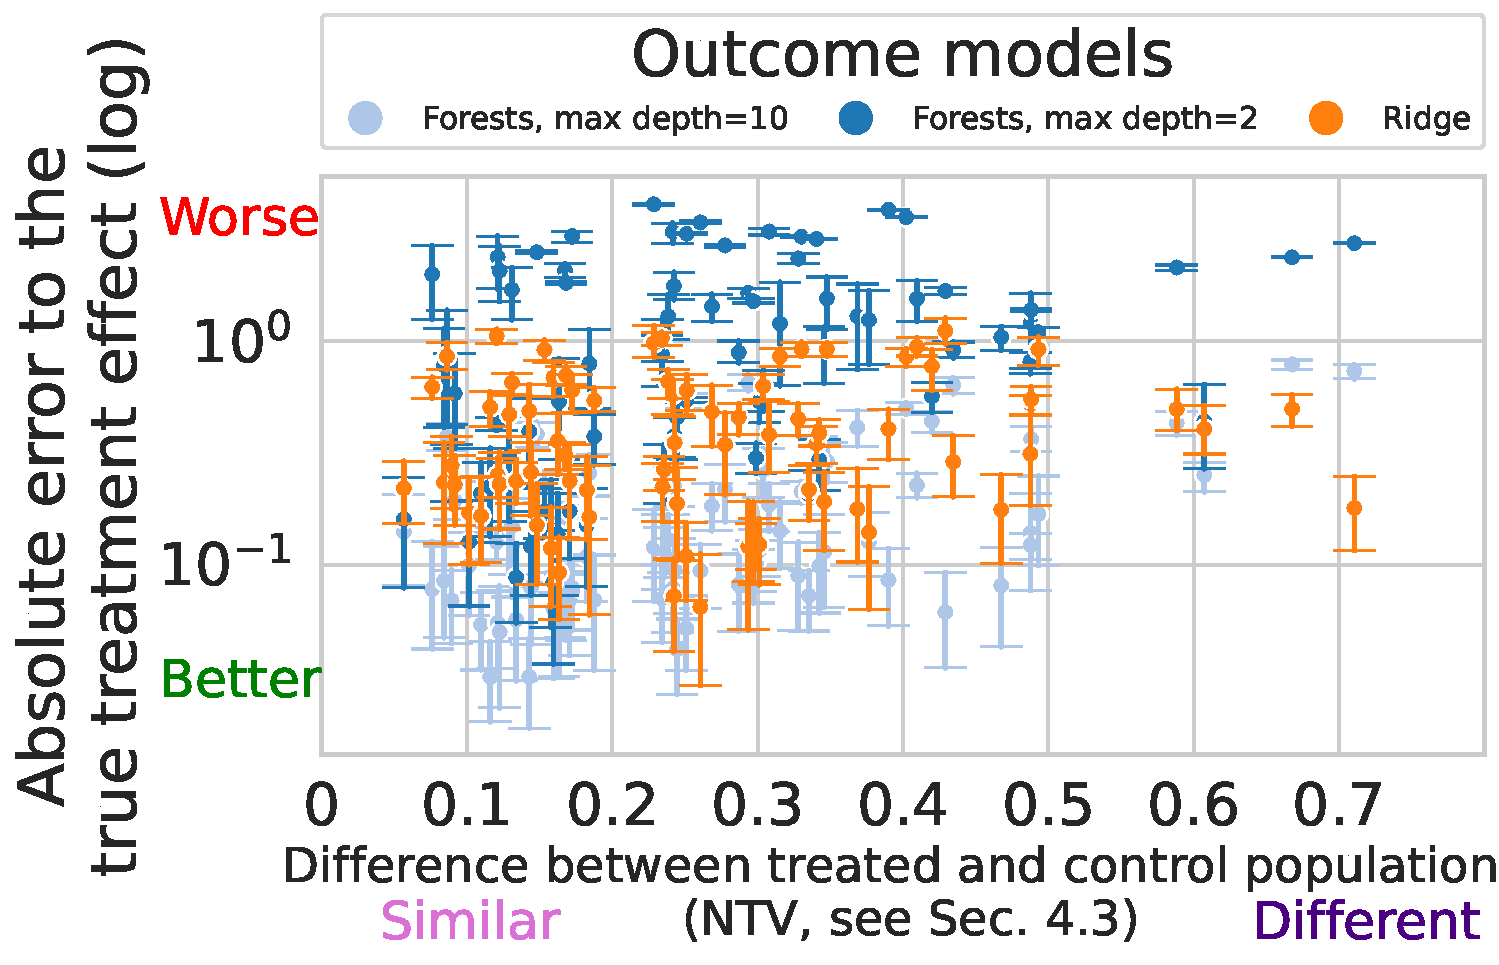
\includegraphics[width=0.8\linewidth]{img/chapter_5/_2023-03-08-11-10-28_acic_2016_ate_heterogeneity.parquet_abs_bias_ylog_scale=True.pdf}%
  \caption{\textbf{Different outcome models lead to different
      estimation errors on the Average Treatment Effects},
    on 77 classic simulations with known true causal effect
    \citep{dorie_automated_2019}. The different models are ridge regression
    and random forests with different hyper-parameters
    (details
    \ref{apd:toy_example:acic_2016_ate_variability}). The different configurations are
    plotted as a function of increasing difference between treated and
    untreated population --see
    \autoref{subsec:measuring_overlap}.
    There is no systematic best performer; data-driven model
    selection is important.
    \label{fig:acic_2016_ate_heterogeneity}%
  }
\end{figure}

Standard practices to select models in predictive settings rely on
the error on the outcome
\citep{poldrack2020establishment,varoquaux2022evaluating}. However, as we
will see, these practices may not pick the best models
for causal inference, as they can be misled by inhomogeneities due to
treatment allocation.
%
Given complex, potentially noisy, data, which model is to be most trusted to
yield valid causal estimates? As no single learner performs
best on all data sets, there is a pressing need for clear guidelines to select
outcome models for causal inference.

\paragraph{Objectives and structure of the paper}

In this paper, we study \textit{model selection procedures}
in practical settings: \textit{finite samples} settings and without
\textit{well-specification} assumption. Asymptotic causal-inference
theory calls for complex risks, but a practical question is
whether model-selection procedures, that rely on data split, can estimate
these risks reliably enough. Indeed, they
come with more quantities to estimate, which may
bring additional variance, leading to worse model selection.

We first illustrate the problem of causal model
selection and briefly review prior art. Then, Section
\ref{sec:framework} sets causal model selection in the
\emph{potential outcome} framework and details the causal risks and
model-selection procedure. Section \ref{sec:theory} gives theoretical
results. Section \ref{sec:empirical_study} details a thorough empirical
study, covering many different settings. Finally, Section \ref{sec:discussion}
discusses the findings.
%
Results outline how to best select outcome models for causal
inference with an adapted
cross-validation to estimate the so-called $R\mathrm{-risk}$.
This risk compensates for systematic
differences between treated and non-treated individuals using
two \emph{nuisance} models,
themselves estimated from data and thus imperfect; yet these
imperfections do not undermine the $R\mathrm{-risk}$.

% XXX: merge the two paragraphs, above and below

Illustration: the best predictor may not estimate best causal effects
Prior work: model selection for outcome modeling (g-computation)


\subsection{Prior work: model selection for outcome modeling (g-computation)}%


A natural way to select a predictive model for causal inference would be
an error measure between a causal quantity such as the CATE and models' estimate. But such error is
not a ``feasible'' risk: it cannot be computed solely from observed data
and requires oracle knowledge.

% XXX: I think that I should make the following paragraph shorter

\paragraph{Simulation studies of causal model selection}

Using eight simulations setups from \cite{powers_methods_2018}, where
the oracle CATE is known, \citet{schuler_comparison_2018} compare four
causal risks, concluding that for CATE estimation the best
model-selection risk is the so-called $R\text{-risk}$
\cite{nie_quasioracle_2017} --def.\,\ref{def:r_risk}, below. Their
empirical results are clear for randomized treatment allocation but less
convincing for observational settings where both simple Mean Squared
Error --MSE, $\mu\text{-risk}(f)$ def.\,\ref{def:mu_risk}-- and
reweighted MSE --$\mu\text{-risk}_{IPW}$ def.\,\ref{def:mu_ipw_risk}--
appear to perform better than $R\text{-risk}$ on half of the simulations.
Another work \cite{alaa_validating_2019} studied empirically both MSE and
reweighted MSE risks on the semi-synthetic ACIC 2016 datasets
\cite{dorie_automated_2019}, but did not include the $R\text{-risk}$. We complete these
prior empirical work by studying a wider variety of data generative
processes and varying the influence of overlap, an important parameter of
the data generation process which makes a given causal metric appropriate
\cite{damour_overlap_2020}. We also study how to best adapt
cross-validation procedures to causal metrics which themselves come with
models to estimate.

\paragraph{Theoretical studies of causal model selection}

Several theoretical works have proposed causal model selection procedures
that are \emph{consistent}: select the best model in a family given
asymptotically large data. These work rely on introducing a
CATE estimator in the testing procedure: matching
\citep{rolling_model_2014}, an IPW estimate
\citep{gutierrez_causal_2016}, a doubly robust estimator
\citep{saito_counterfactual_2020}, or debiasing the error with influence
functions \cite{alaa_validating_2019}. However, for theoretical
guarantees to hold, the test-set correction needs to converge to the
oracle: it needs to be flexible enough --well-posed-- and asymptotic
data. From a practical perspective, meeting such requirements
implies having a good CATE estimate, thus having solved
the original problem of causal model selection.

\paragraph{Statistical guarantees on causal estimation procedures}

Much work in causal inference has focused on procedures that
guarantee asymptotically consistent estimators, such as Targeted
Machine Learning
Estimation (TMLE) \cite{laan_targeted_2011,schuler_targeted_2017} or
Double Machine Learning \cite{chernozhukov_double_2018}. Here also, theories require asymptotic regimes and
models to be \textit{well-specified}.

By contrast, \citet{johansson2022generalization} studies causal estimation
without assuming that estimators are well specified. They derive an upper bound
on the oracle error to the CATE ($\tau\text{-risk}$) that involves the error on
the outcome and the similarity of the distributions of treated and control
patients. However, they use this upper bound for model optimization,
and do not give insights on model selection. In addition, for hyperparameter
selection, they rely on a plugin estimate of the $\tau\text{-risk}$ built with
counterfactual nearest neighbors, which has been shown ineffective
\cite{schuler_comparison_2018}.

\section{Formal setting: causal inference and model selection}\label{sec:framework}

\subsection{The Neyman-Rubin Potential Outcomes framework}%
\label{sec:neyman_rubin}%

\paragraph{Settings}

The Neyman-Rubin Potential Outcomes framework
\cite{naimi2023defining,imbens_causal_2015} enables statistical reasoning on
causal treatment effects: Given an outcome $Y \in \mathbb R$ (eg. mortality risk
or hospitalization length), function of a binary treatment $A \in \mathcal{A} =
  \{0, 1\}$ (eg.~a medical procedure, a drug administration), and baseline
covariates $X \in \mathcal{X} \subset \mathbb{R}^d$, we observe the factual
distribution, $O = (Y(A), X, A) \sim \mathcal D = \mathbb P(y, x, a)$. However,
we want to model the existence of potential observations (unobserved ie.
counterfactual) that correspond to a different treatment. Thus we want
quantities on the counterfactual distribution $O^{*} = (Y(1), Y(0), X, A) \sim
  \mathcal D^{*} = \mathbb P(y(1), y(0), x, a)$.

Popular quantities of interest (estimands) are:
at the population level, the
Average Treatment Effect
\begin{flalign*}
  \text{ATE} &  &
  \tau \myeq \; \mathbb{E}_{Y(1),Y(0) \sim \mathcal D^*}[Y(1) - Y(0)];
             &  &
\end{flalign*}
at the individual level, to model heterogeneity, the Conditional Average Treatment Effect
\begin{flalign*}
  \text{CATE} &  &
  \tau (x) \myeq \; \mathbb{E}_{Y(1),Y(0) \sim \mathcal{D}^\star}[Y(1) - Y(0) | X=x].
              &  &
\end{flalign*}

\paragraph{Causal assumptions}

Assumptions are necessary for causal estimands to be
identifiability
in observational settings \cite{rubin_causal_2005}. We assume the usual
strong ignorability assumptions: \emph{1)}
\emph{unconfoundedness} \mbox{$\{Y(0),
    Y(1) \} \indep A | X$}, \emph{~2)} \emph{strong overlap} ie. every patient has a
strictly positive probability to receive each treatment, \emph{3)}
\emph{consistency}, and \emph{4)} \emph{generalization} (detailed in
\ref{apd:causal_assumptions}).

\paragraph{Estimating treatment effects with outcome models}\label{subsec:estimators}

Should we know the two expected outcomes for a given $X$,
we could compute the
difference between them, which gives the causal effect of the treatment.
%
These two expected outcomes can be computed from the observed data:
the consistency \ref{assumption:consistency} and unconfoundedness
\ref{assumption:ignorability} assumptions imply the equality of two different
expectations:
\begin{equation}\label{eq:mu_identification}
  \mathbb E_{Y(a) \sim \mathcal{D^{\star}}} [Y(a)|X=x] = \mathbb E_{Y \sim \mathcal{D}} [Y|X=x, A=a]
\end{equation}
On the left, the expectation is taken on the counterfactual unobserved
distribution. On the right, the expectation is taken on the factual observed
distribution conditionally on the treatment. This equality is referred as the
g-formula identification \cite{robins_new_1986}. For the rest of the
paper, the expectations will always be taken on the factual observed
distribution $\mathcal{D}$. This identification leads to outcome based estimators (ie.
g-computation estimators \cite{snowden_implementation_2011}), targeting the
ATE $\tau$ with outcome modeling:
\begin{eqnarray}
  \tau =& \mathbb E_{Y \sim \mathcal{D^{\star}}}[Y(1) - Y(0)|X=x]
  \notag
  \\
  = &\mathbb E_{Y \sim \mathcal{D}}[Y|A=1] - \mathbb E_{Y \sim \mathcal{D}}[Y| A=0]
  \label{eq:tau_population}
\end{eqnarray}
This equation builds on two quantities: the conditional expectancy
of the outcome given the covariates and either
treatment or no no treatment, called \emph{response function}:
\begin{flalign*}
  \text{Response function}
   &  &
  \mu_{a}(x) \myeq \; \mathbb E_{Y \sim \mathcal{D}} [Y|X=x, A=a]
   &  &
\end{flalign*}

Given a sample of data and the oracle response functions $\mu_0, \mu_1$, the
finite sum version of \autoref{eq:tau_population} leads to an
estimator of the ATE written:
\begin{equation}
  \hat \tau = \frac{1}{n} \biggl(\sum_{i=1}^n \mu_{1}(x_i) - \mu_{0}(x_i) \biggr)
  \label{eq:ate_estimate}
\end{equation}
This estimator is an oracle \textbf{finite sum estimator} by opposition to the
population expression of $\tau$, $\mathbb{E}[\mu_{1}(x_i) - \mu_{0}(x_i)]
$,
which involves an expectation taken on the full
distribution $\mathcal D$, which is observable but requires infinite data. For
each estimator $\ell$ taking an expectation over $\mathcal D$, we use the symbol
$\hat \ell$ to note its finite sum version.

Similarly to the ATE, at the individual level, the CATE:
\begin{equation}
  \tau(x) = \mu_{1}(x) - \mu_{0}(x)
  \label{eq:cate_estimate}
\end{equation}

\paragraph{Robinson decomposition}
The \emph{R-decomposition}
of the outcome model plays an important role,
\cite{robinson_rootnconsistent_1988}:
introducing two quantities, the conditional mean outcome
and the probability to be treated (known as propensity score \cite{rosenbaum_central_1983}):
\begin{flalign}
  \text{Conditional mean outcome} &                    & m(x) \myeq \; & \mathbb E_{Y \sim
  \mathcal{D}} [Y|X=x]            &                    &
  \label{def:m}
  \\
  \text{Propensity score}         &                    &
  e(x) \myeq \;                   & \mathbb P[A=1|X=x]
  \label{def:propensity_score}
\end{flalign}
the outcome can be written
\begin{flalign}\label{eq:r_decomposition}
  \text{R-decomposition}            &  & y(a) = m(x) + \big( a - e(x) \big)
  \tau(x) + \varepsilon(x; a)\notag &  &
  \\\ &&\text{with}\quad \mathbb E[\varepsilon(X; A)|X, A] = 0&&
\end{flalign}
$m$ and $e$ are often called
\emph{nuisances} \cite{chernozhukov_double_2018}; they are unknown.

%As noted by \cite{johansson2022generalization}, the machine learning
%community often referred to the CATE by ITE, the Individual Treatment Effect.
%From a purely causal point of view, the ITE is uniquely defined for each
%individual and might not be accessible: $ITE(x_i) = Y_i(1) -  Y_i(0)$. On the
%contrary, the CATE can always be derived by taking conditional expectancies. It
%is the expected effect of the treatment in the region of the covariate space
%around X. %Too cultivate

\begin{table*}[!tb]
  \makebox[\linewidth]{
    \begin{threeparttable}[b]
      \caption{Review of causal risks
        ---
        The $R\text{-risk}^*$ is called $\tau \text{-risk}_R$ in
        \citet{schuler_comparison_2018}.
        \label{tab:evaluation_metrics}}
      \centering
      \begin{tabular}{llr}
        \toprule
        Risk                                                                                           & Equation
                                                                                                       & Reference                                                                                                                                           \\
        \midrule
        $mse(\tau(X), \tau_f(X))=\tau\text{-risk}$                                                     & $\mathbb E_{X\sim
              p(X)}[(\tau(X) - \hat \tau_f(X))^2] $
                                                                                                       & Eq. \ref{eq:tau_risk} \cite{hill_bayesian_2011}                                                                                                     \\
        $mse(Y, f(X)) = \mu\text{-risk}$                                                               & $\mathbb{E}_{(Y, X, A)
            \sim \mathcal D}\left[(Y-f(X ; A))^2 \right]$
                                                                                                       & Def. \ref{def:mu_risk} \cite{schuler_comparison_2018}                                                                                               \\
        $\mu\text{-risk}_{IPW}^*$                                                                      & $\mathbb{E}_{(Y, X, A)
            \sim \mathcal D}\left[ \Big( \frac{A}{e(X)} + \frac{1-A}{1-e(X)} \Big)
        (Y-f(X ; A))^2 \right]$                                                                        & Def.
        \ref{def:mu_ipw_risk} \cite{vanderlaan_unified_2003}                                                                                                                                                                                                 \\
        $\tau\text{-risk}^{\star}_{IPW}$                                                               & $\mathbb{E}_{(Y, X, A) \sim \mathcal D} \left[ \Big(Y \left( \frac{A}{e(X)} - \frac{1-A}{1-e(X)}\right)-\hat \tau_f\left(X\right)\Big)^2 \right]$ &
        Def. \ref{def:tau_ipw_risk} \cite{wager_estimation_2018}
        \\
        $U\text{-risk}^*$                                                                              & $\mathbb{E}_{(Y, X, A) \sim \mathcal D}  \big[
        \big( \frac{Y-m\left(X\right)}{A-e\left(X\right)} -  \hat \tau_f\left(X\right)\big)^{2} \big]$ &
        Def. \ref{def:u_risk} \cite{nie_quasioracle_2017}
        \\
        $R\text{-risk}^*$                                                                              & $\mathbb{E}_{(Y, X, A)
            \sim \mathcal D} \big[\big(\left(Y-m\left(X\right)\right)
        -\left(A-e\left(X\right)\right) \hat \tau_f\left(X\right)\big)^{2} \big]$                      &
        Def. \ref{def:r_risk} \cite{nie_quasioracle_2017}
        \\
        \bottomrule
      \end{tabular}
    \end{threeparttable}
  }
\end{table*}


\section{Methods}\label{sec:causal_model_selection:methods}




\subsection{Notations}\label{subsec:causal_model_selection:notations}

\subsection{Model-selection risks, oracle and feasible}\label{subsec:causal_model_selection:risks}
\subsection{Causal model selection}\label{subsec:causal_model_selection:causal_model_selection}

The $\tau\mathrm{-risk}$ : an oracle error risk
Feasible error risks
Estimation and model selection procedure
\section{Theory: Links between feasible and oracle risks}\label{sec:causal_model_selection:theory}

\subsection{Upper bound of $\tau\mathrm{-risk}$ with
  $\mu\mathrm{-risk}_{IPW}$}\label{subsec:causal_model_selection:upper_bound}

\subsection{Reformulation of the R-risk as reweighted
  $\tau\mathrm{-risk}$}\label{subsec:causal_model_selection:r_risk_reformulation}

\subsection{Interesting special
  cases}\label{subsec:causal_model_selection:special_cases}

\section{Empirical Study}\label{sec:causal_model_selection:empirical_study}

\subsection{Caussim: Extensive simulation settings}\label{subsec:causal_model_selection:caussim}
\paragraph{Data Generation Process}

Family of candidate estimators

\subsection{Semi-simulated datasets}\label{subsec:causal_model_selection:semi_simulated}
\paragraph{Datasets}
\paragraph{Family of candidate estimators}
\paragraph{Nuisance estimators}

\subsection{Measuring overlap between treated and non treated}\label{subsec:causal_model_selection:overlap}

\subsection{Empirical results: factors driving good model selection across
  datasets}\label{subsec:causal_model_selection:empirical_results}


The $R\mathrm{-risk}$ is the best metric

Model selection is harder in settings of low population overlap

Nuisances can be estimated on the same data as outcome
models

Use 90\% of the data to estimate outcome models, 10\% to select them

\section{Discussion and conclusion}\label{sec:causal_model_selection:discussion}


\chapter{Conclusion}\label{chapter:conclusion}

%Healthcare burden in modern world is access to healthcare, and chronic disease
%ie. resource issues more than better products, our methodological toolbox to
%distinguish between good and bad management is not adapted to the task since it
%involved complicated process specific to each situation. Some can be borrowed
%from economics, but specificities from epidemiology should be mixed in. 
Modern healthcare burdens and costs are driven by chronic diseases where death
is not the only outcome of interest. Focus on smaller rewards, on which
experiments are easier to conduct and where error is possible: it would allow
better learning for decision making since we can repeat more experiments (limit:
signals could be highly delayed).

% Pattern exists in the massive data collected: we need to extract them
% automatically and articulate these with scientific questions guided by
% knowledge domain.
Text is pervasive, we are using it to communicate and to log most of our
information. We can rely pretraining models outside the healthcare domain. We
should leverage it more in the context of care (limit: temporality is hard to
capture but is a key aspect of causal inference).

% Those problem are more pragmatic than theoretical. Thus, data and conclusions need to circulate. 
The unreasonable effectiveness of healthcare data is yet out of reach due to
hugely difficult transfer of models or administrative barriers to access data
(due to multiplicity of the involved actors). This forces us to rely on
efficient techniques that make the best of medium-sized data or rely on sharable
sources of knowledge (aggregated statistics, federated learning approaches,
ontologies, ...).


\printbibliography

\clearpage
\begin{appendices}
  \section{Statistical models}\label{apd:statistical_models}

  \section{Causal Diagrams}\label{apd:causal_diagrams}

\end{appendices}
\end{document}
